\قسمت{دیدهای مولفه و اتصال}
\زیرقسمت{دید سطح اول}
\begin{figure}[H]
\centering
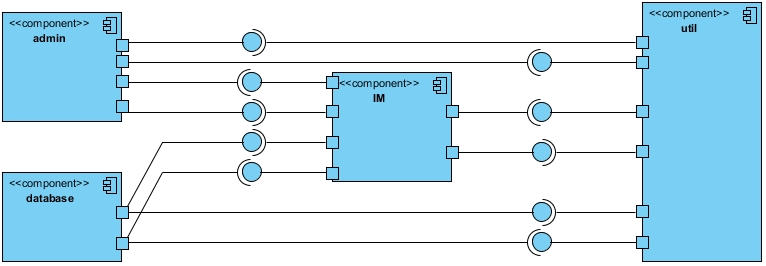
\includegraphics[scale=.4]{img/lvl1.jpg}
\caption{\lr{IM C\&C View}}

\end{figure}
\زیرقسمت{مولفه IM}
\زیرزیرقسمت{دید اصلی}
\begin{figure}[H]
\centering
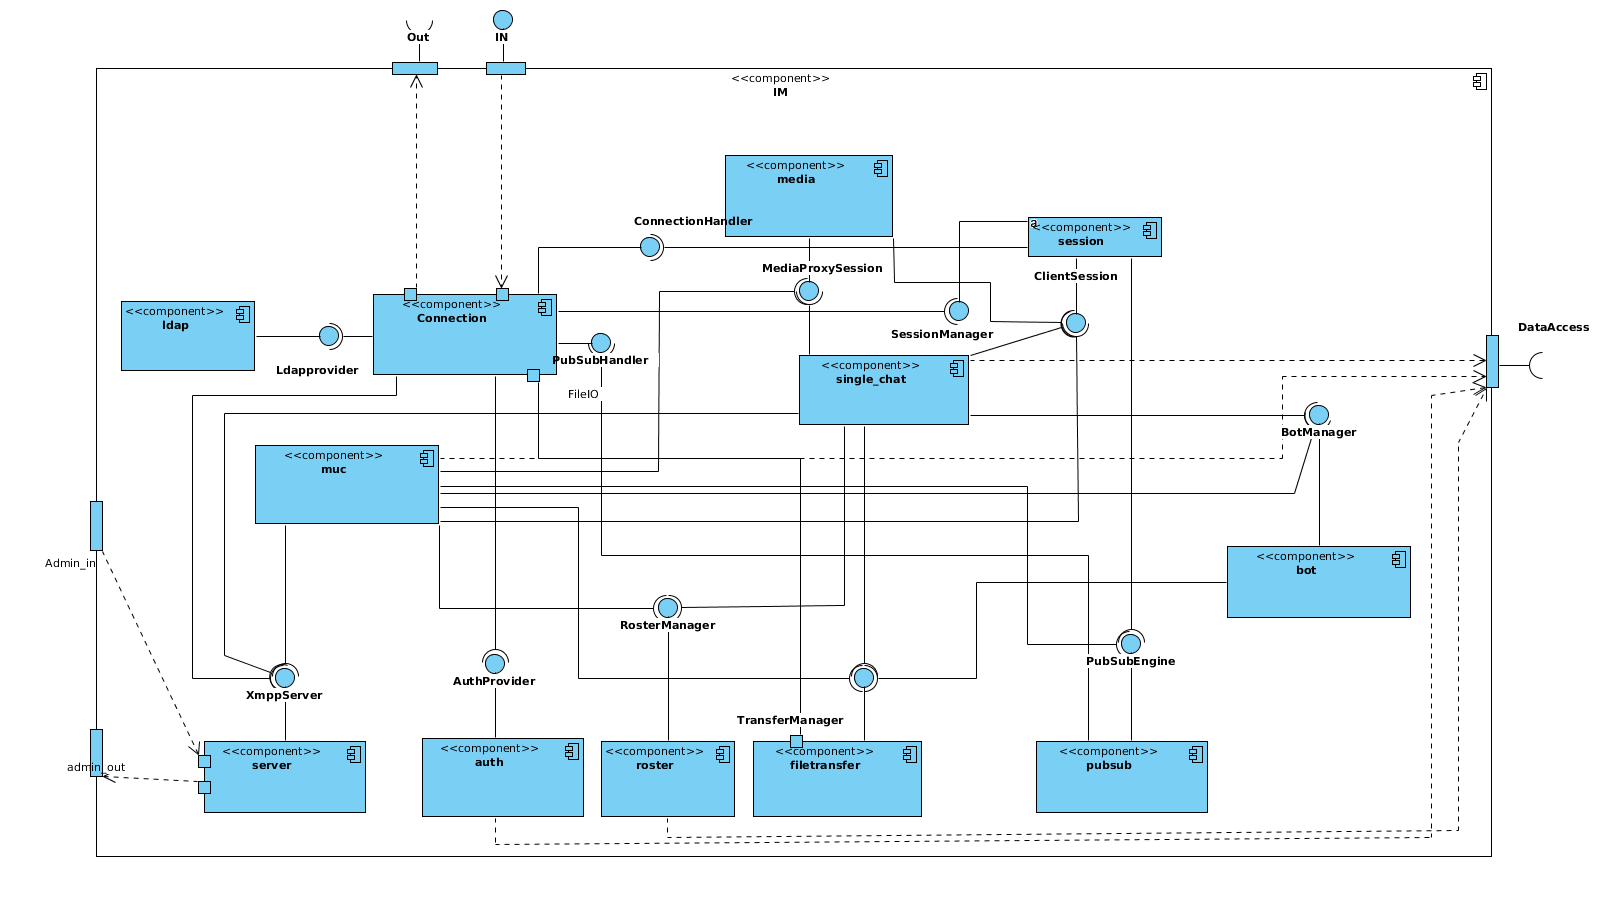
\includegraphics[scale=.28]{img/im.png}
\caption{\lr{IM C\&C View}}

\end{figure}
\زیرزیرقسمت{عناصر}
\begin{itemize}

\فقره Server : این مولفه مسؤولیت مقداردهی اولیه و برپایی مولفه‌های connection ، muc و singlchat را برعهده دارد. همچنین با مولفه‌ی بیرونی admin تعامل دارد.
\فقره muc : این مولفه عملیات‌های مربوط به چت گروهی را بر عهده دارد.
\فقره singlechat : چت دو نفره در این مولفه پشتیبانی می‌شود. 
\فقره connection :  انواع مختلفی از ارتباطات با محیط بیرون را سازماندهی می‌کند.
\فقره auth : وظایف مربوط به احراز هویت افراد در این مولفه انجام می‌گیرد.
\فقره roster : فهرست‌های مختلفی را نگهداری می‌کند. مانند فهرست مخاطبین فرد، فهرست افراد یک گروه.
\فقره filetransfer : تبادل فایل به وسیله‌ی این مولفه انجام می‌گیرد. این فایل ها در متن چتها تبادل می‌شود.
\فقره  pubsub : پیاده سازی الگوی publish-subscribe که اطلاع رسانی رویدادها را بر عهده دارد. 
\فقره bot : عملیات‌های مربوط به رباتها در این مولفه قرار دارد.
\فقره ldap : دسترسی به اطلاعات مکان افراد یا اشیاء در این مولفه قرار داد. 
\فقره session : تعامل کاربران با سامانه از طریق این مولفه صورت می‌گیرد.
\فقره media : امور رسانه‌ای مانند عکسهای موجود در حساب کاربری و تماس صوتی یا تصویری در این قسمت قرار می‌گیرد.
\end{itemize}



\زیرقسمت{مولفه database}

\زیرزیرقسمت{دید اصلی}
\begin{figure}[H]
\centering
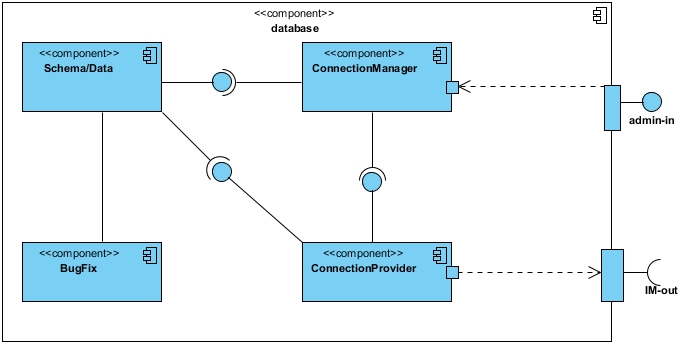
\includegraphics[scale=.5]{img/database.jpg}
\caption{\lr{database C\&C View}}

\end{figure}

\زیرزیرقسمت{عناصر}

\begin{itemize}

	

	\فقره schemadata : این مولفه مسؤولیت مدریت شِما و  داده‌ها را دارد و تغییرات و به روز رسانی‌های آن و اطمینان از به روز بودن پایگاه داده نسبت به شما را بر عهده دارد. 

	\فقره bugfix :  این مولفه در مواردی در صورت لزوم به مشکلاتی که رخ می‌دهند رسیدگی می‌کند.

	\فقره connectionmanager :  مدیریت ارتیاظ‌هایی که با پایگاه داده برقرار می‌شود را بر عهده دارد.

	\فقره connectionprovider : وظیفه فراهم‌سازی ارتباط برای مولفه‌های دیگر با دیتابیس را بر عهده دارد.

	

\end{itemize}





\زیرقسمت{مولفه util}

\زیرزیرقسمت{دید اصلی}
\begin{figure}[H]
\centering
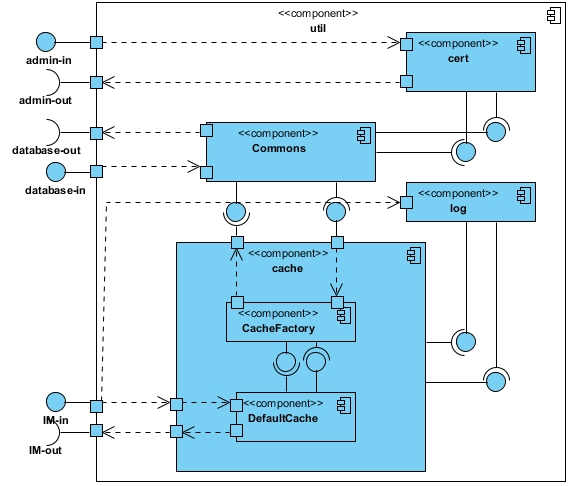
\includegraphics[scale=.5]{img/util.jpg}
\caption{\lr{util C\&C View}}

\end{figure}

\زیرزیرقسمت{عناصر}

\begin{itemize}



\فقره cert : این مولفه مسؤولیت مدریت یک سری اختیارات و گواهی‌های صادر شده از سوی مدیر را به عهده دارد.

\فقره log :  این مولفه تاریخچه‌ی درخواست‌هایی که به حافظه سیستم می‌آید و دسترسی‌هایی که انجام می‌شود را نگه می‌دارد.

\فقره cache : این مولفه داده‌هایی که نیاز است را در خود نگه می‌دارد.

\فقره defaultcache : این مولفه داده‌هایی که در حافظه موجود است را ارائه می‌د‌هد.

\فقره cachefactory : این مولفه داده‌هایی که نیاز است از پایگاه داده می‌گیرد و در حافظه ذخیره می‌کند.

\فقره commons : وظیفه تبادل داده‌ها با پایگاه داده را بر عهده دارد.



\end{itemize}



\زیرقسمت{مولفه admin}


\زیرزیرقسمت{دید اصلی}
\begin{figure}[H]
\centering
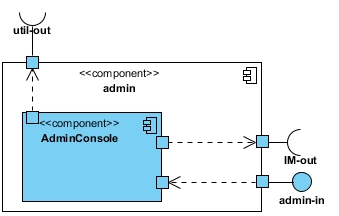
\includegraphics[scale=.5]{img/admin.jpg}
\caption{\lr{admin C\&C View}}

\end{figure}
\زیرزیرقسمت{عناصر}

\begin{itemize}

	

	\فقره adminconsole : یک سری اختیارات خاص در اختیار مدیران قرار می‌دهد مثل دسترسی به پایگاه‌داده و ایجاد یک سری تغییرات.



\end{itemize}



\زیرزیرقسمت{نمودار Context}


\begin{figure}[H]
\centering
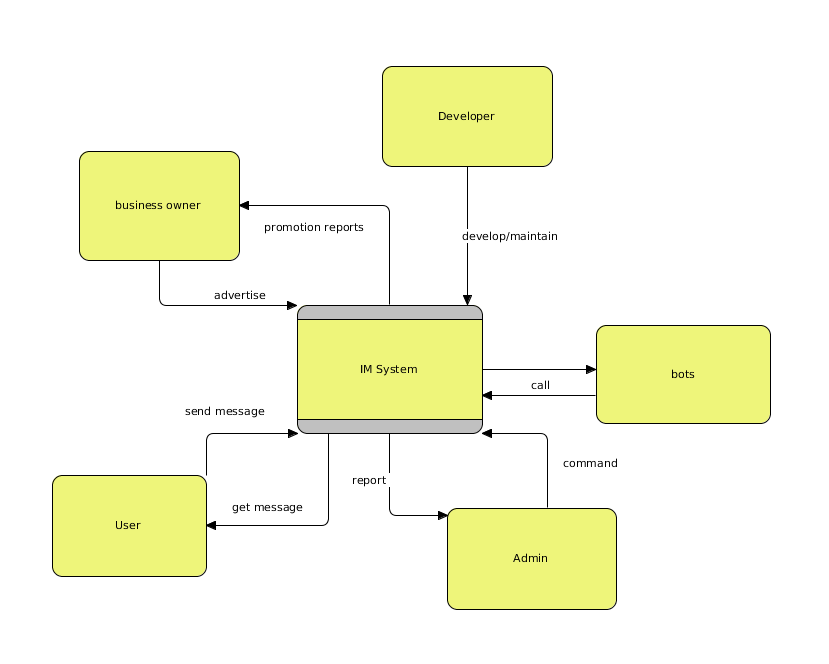
\includegraphics[scale=.5]{img/context.png}
\caption{\lr{Context Diagram}}

\end{figure}


\زیرقسمت{نیازمندی‌های کارکردی}

در این بخش به بیان نیازمندی‌های کل سیستم خواهیم پرداخت. همانطور که در زیر می‌بینید کل سیستم در سطح اول به چندین مولفه تقسیم می‌شود که در زیر برای هر یک از این مولفه‌ها و زیر مولفه‌هایشان نیازمندی‌های کارکردی را بیان می‌کنیم که در مجموع کل نیازمندی‌های کارکردی سیستم را پوشش می‌دهد.
\زیرزیرقسمت{IM}
\begin{itemize}
\فقره ldap : 
\begin{itemize}
\فقره مکان‌یابی افراد
\فقره مکان‌یابی منابع مانند فایلها در شبکه 
\end{itemize}
\فقره   connection :
\begin{itemize}
\فقره  مدیریت ارتباطات ورودی و خروجی
\فقره فراهم آوردن بستر مناسب جهت برقراری ارتباط با انواع پروتکل‌های مناسب
\end{itemize}
\فقره media : 
\begin{itemize}
	\فقره ایجاد تماس صوتی در چت دو تفره
	\فقره ایجاد تماس تصویری در چت دو تفره
	\فقره فراهم سازی و مدیریت تصاویر مربوط به حساب های کاربری
	
\end{itemize}
\فقره  session :
\begin{itemize}
	\فقره سازماندهی ارتباطات کاربران با سرور در حالت نیمه پایدار
	\فقره ارتباط با مولفه های مربوط به چت به منظور فراهم کردن عملکردهای پیام رسان
	\فقره اطلاع از وضعیت کاربران
	\فقره ذخیره‌ی اطلاعات تعاملات
\end{itemize}

\فقره muc : 
\begin{itemize}
\فقره ایجاد گروه به منظور چت گروهی
\فقره ایجاد کانال
\فقره تبادل پیام در گروه و کانال
\فقره مدیریت تبلیغات در کانال‌ها
\فقره دریافت داده از ربات‌ها و انتشار
\فقره ذخیره محتواهای چتها و کانالها
\end{itemize}

\فقره singlechat :

\begin{itemize}
\فقره ایجاد مکالمه جهت چت دو نفره
\فقره تبادل پیام در چت
\فقره دریافت داده از ربات‌ها و انتشار
\فقره ذخیره محتواهای چت 

\end{itemize}
\فقره bot : 
\begin{itemize}
\فقره فراهم ساختن سرویس‌های لازم جهت ساخت ربات
\فقره ارسال دستور به ربات ها
\فقره دریافت و انتشار پاسخ ربات ها
\end{itemize}

\فقره pubsub :
\begin{itemize}
\فقره انتشار وضعیت کاربران ماننذ آنلاین بودن
\فقره انتشار رویدادها
\end{itemize}
\فقره  filetransfer : 
\begin{itemize}
\فقره انتقال فایل در محیط چت دو نفره
\فقره انتقال فایل در محیط گروه و کانال نفره
\end{itemize}
\فقره roster :
\begin{itemize}
\فقره نگهداری لیست مخطبین کاربران
\فقره نگهداری لیست اعضای گروه
\فقره نگهداری لیست اعضای کانال
\end{itemize}

\فقره auth: 
\begin{itemize}
\فقره مدیریت حسابهای کاربری
\فقره ایجاد حساب کاربری جدید
\فقره احراز هویت افراد
\فقره مشخص کردن میزان دسترسی افراد
\end{itemize}
\فقره server :
\begin{itemize}
\فقره مقداردهی و آماده سازی مولفه‌های connection ، muc ، singlechat
\فقره اجرا کردن دستورات admin در رابطه با نحوه‌ی کار پیام رسانی
\end{itemize}
\end{itemize}

\زیرزیرقسمت{database}


\begin{itemize}	

	\فقره schemadata : 

	\begin{itemize}	

		\فقره	مدیریت کردن شِما و پایگاه داده

		\فقره	مدیریت  کردن تغییرات  شِما و پایگاه داده

		\فقره	مدیریت  کردن به روزرسانی‌های شِما و پایگاه داده

		\فقره 	اطمینان حاصل کردن از تطابق پایگاه‌داده با شما 

		\فقره	پاسخ به پرس‌وجوها

		

	\end{itemize}

	\فقره bugfix :

	\begin{itemize}	

		

		\فقره کشف کردن خطاهای مولفه دیتابیس

		\فقره یافتن منشا ارور

	   \فقره نشان دادن واکنش مناسب به خطای مربوطه مثل پیام خطای مناسب و یا تصحیح مناسب

		

	\end{itemize}

	\فقره connectionmanager :

	\begin{itemize}

	   \فقره دریافت کردن درخواست‌های مولفه‌های دیگر برای برقراری ارتیاط با پایگاه‌داده

		\فقره حصول اطمینان از امنیت درخواست‌ها

		\فقره ارسال کردن درخواست‌های مطمئن به پایگاه‌داده

		\فقره ممانعت ا ارسال درخواست‌های مشکوک

		\فقره حفظ ترتیب درخواست‌ها

	\end{itemize}

	

	\فقره connectionprovider : 

	\begin{itemize}

		\فقره ارسال کردن پاسخ‌های مناسب به مولفه‌های مناسب

		\فقره حفظ ترتیب ارسال‌ها

		

	\end{itemize}	

\end{itemize}



\زیرزیرقسمت{util}

\begin{itemize}	

	\فقره cert : 

	\begin{itemize}	

		\فقره	دریافت کردن درخواست‌های مدیر

		\فقره	بررسی کردن درخواست‌های مدیر

	   \فقره	جدا کردن درخواست‌های ایمن و معتبر از غیرایمن و نامعتبر

		\فقره 	ثبت درخواست‌های معتبر در پایگاه داده

		

	\end{itemize}

	\فقره log :

	\begin{itemize}	

		

		\فقره دریافت درخواست‌های حافظه‌ای

		\فقره دریافت پاسخ‌های حافظه‌ای

	   	\فقره ایجاد تاریخچه از روی آن‌ها

		

	\end{itemize}

	\فقره cache :

	\begin{itemize}

	    \فقره دریافت کردن درخواست‌های دسترسی به داده

		\فقره ذخیره داده‌های پراستفاده و محلی

		\فقره پاسخ به درخواست‌های دریافتی

		

	\end{itemize}

	

	\فقره defaultchache : 

	\begin{itemize}

		\فقره دریافت درخواست داده از مولفه‌ها

		\فقره بررسی درخواست و اطمینان از سلامت و ایمنی آن

		\فقره جستجو در حافظه

		\فقره پاسخ به درخواست دریافتی در صورت وجود داده درخواستی

	   \فقره ارسال پیام مبتنی بر عدم وجود به  cachefactory در صورت عدم وجود داده درخواستی در حافظه

	    \فقره دریافت ack از cachefactory مبنی بر وجود داده درخواستی

		\فقره پاسخ به درخواست مولفه مربوطه 

	\end{itemize}	

	

\فقره chachefactory : 

\begin{itemize}

	\فقره دریافت پیام‌های defaultchache

	\فقره ارسال درخواست به مولفه common

	\فقره دریافت پاسخ از common   

	\فقره ثبت داده در حافظه

	\فقره ارسال ack برای chachefactory مبنی بر وجود داده درخواستی در حافظه

\end{itemize}	





	

\فقره chachefactory : 

\begin{itemize}

	\فقره دریافت پیام‌های defaultchache

	\فقره ارسال درخواست به مولفه common

	\فقره دریافت پاسخ از common   

	\فقره ثبت داده در حافظه

	\فقره ارسال ack برای chachefactory مبنی بر وجود داده درخواستی در حافظه

\end{itemize}	



	

\فقره common : 

\begin{itemize}

	\فقره دریافت پیام‌های مولفه‌های مختلف کش

	\فقره اطمینان از سالم و ایمن بودن درخواست‌ها

	\فقره ارسال درخواست به پایگاه‌داده

	\فقره دریافت پاسخ پایگاه داده

	\فقره ارسال پاسخ به مولفه مربوطه

\end{itemize}	



\end{itemize}

\زیرزیرقسمت{admin}

\begin{itemize}	

	\فقره adminconsole : 

	\begin{itemize}	

		 \فقره	تعامل با مدیر

		\فقره	ارسال درخواست‌های مدیر به مولفه util	یا مولفه‌های دیگر

		 \فقره 	دریافت پاسخ‌ها و نمایش آ‌ن‌ها به مدیر

		

	\end{itemize}

\end{itemize}	




\زیرقسمت{نیازمندی‌های کیفی}



مشخص است که در بخش نیازمندی‌های کارکردی، مشخصه‌هایی که درنظرگیرنده‌ی کیفیت سامانه هستند جایی ندارند. لذا در این بخش به همان روش بالا و بر حسب همان دسته‌بندی دو سطحی که مشاهده کردید به مشخصه‌های کیفی سیستم پرداخته‌ایم، بدین گونه که آن‌ها را در قالب چگونگی ارتباط مولفه‌ها با یکدیگر توضیح خواهیم داد. علاوه بر این در یک بخش اضافه بر بخش‌های قبلی ارتباطات بین مولفه‌های سطح یک را نیز بررسی خواهیم کرد.







\زیرزیرقسمت{ارتباطات بین مولفه‌های سطح اول سامانه(مولفه‌های اصلی)}



این ارتباطات ارتباطاتی دو طرفه هستند، که بین مولفه های سطح اول سیستم وجود دارند.  ‌در ارتباطاتی که در سطح کلان سیستم داریم مولفه‌های سطح اول به یکدیگر درخواست‌هایی طبق نیاز ارسال می‌کنند و مولفه مقابل نیز پاسخ این درخواست را خواهد داد. نکاتی که بایستی مورد توجه قرار گیرند تا  نیازندی‌های کیفی سیستم در حد مورد انتظار ما باشد در اینجا مطرح خواهند شد. اولین نکته‌ای که مورد توجه است این است که در این معماری از الگوی SOA استفاده شده است. متعاقبا مولفه‌های سیستم پیاده‌سازی‌های کاملا مجزا خواهند داشت و ارتباط مولفه‌ها غالبا از طریق REST خواهد بود. این نکته بیان‌کننده ویژگی‌های ارتباطی ضمنی بود که به انتخاب الگوی ما بازمی‌گشت، حال به سراغ نیازمندی‌های کیفی صریح سیستم می‌رویم. تمامی مولفه‌های سطح اول سیستم بایستی  نیازمندی کیفی کارایی را  پاسخگو باشند، بدون اینکه دچار تاخیر و از کار افتادگی شوند.، ازین رو از هر مولفه چندین نمونه استقرار می‌یابد و  متعادل‌کننده‌ی بار \پانوشت{Loa‌dB‌alancer}  به شکلی بار را تقسیم می‌کند که کارایی و  قابلیت استفاده\پانوشت{Availability} از حد تعیین شده کمتر نشود.از سوی دیگر برای ارتباطاتی که دارای اطلاعات حساس و قابل سو استفاده هستند بایستی تعابیر امنیتی اندیشیده شود تا حداقل‌های نیازمندیِ کیفی امنیت در سیستم حفظ شوند. 

 به عنوان مثال ارتباط  بین admin  و util از یک طرف درخواست‌های ادمین مبنی بر دسترسی به پایگاه داده را به مولفه util منتقل می‌کند، و از طرف دیگر پیامی حاوی نتیجه‌ی درخواستی که مدیر داده است را به مولفه admin بازمی‌گرداند. این فرایند، فرآیندی است که تنها مدیران در آن دخیل هستند. لذا با وجود اینکه معیار های کیفی مثل کارایی نیز بر راحتی مدیران تاثیر می‌گذارد، ولی معیار کیفی حیاتی‌ای که در اینجا با آن دست و پنجه نرم می‌کنیم امینت است. با توجه به فرآیند بسیار حساسی که در اینجا انجام می‌شود و وجود دسترسی‌های به شدت قابل سواستفاده بایستی در خصوص ارتباطات گفته شده بسیار محتاط عمل کنیم و کانال‌های ارتباطی این بخش را شدیدا ایمن سازیم. راهکارهایی مثل رمزگذاری را می‌توانیم برای ایمن‌سازی این بخش مورد استفاده قرار دهیم.




\زیرزیرقسمت{ارتباطات بین مولفه‌های سطح دوم سامانه(مولفه‌های فرعی)}



هر یک از مولفه‌های سطح اول خود از مولفه‌ها و ارتباطات دیگری تشکیل شده‌اند. نیازمندی‌های این مولفه‌ها پیش ازین برررسی شد، حال به ملاحظات معمارانه‌ای که در پس ارتباطات این مولفه‌ها نهفته است می‌پردازیم. تمامی ارتباطات این مولفه‌ها بایستی به شکلی در کنار هم کار کنند که کارایی کلی مولفه‌ای که در آن قرار دارند از مقدار مطلوب کم‌تر نشود. در این نوع ارتباطات نیز کارایی و قابلیت استفاده توسط متعادل کننده بار مدیریت می‌شوند، با این تفاوت که این نکته مورد توجه است که چندین مولفه در کنار هم قرار است کار کنند و یک خروجی را در یک زمان مناسبی تحویل دهند. در واقع مجموع زمان کار و ارتباطات است که اینجا اهمیت می‌یابد و متعادل‌کننده حتما بایستی تاثیرات مولفه‌ها بر یکدیگر را درنظر بگیرد. به عنوان مثال اگر قرار است 5 مولفه پاسخی را در 100 ثانیه بدهند و به طور مثال هر مولفه‌ها 20 ثانیه نیاز داشته باشد و همه یکی پس از دیگری به خروجی قبلی نیاز داشته باشند، در شرایطی که یکی از مولفه‌ها کار خود را در 40 ثانیه انجام می‌دهد خوب است که قابلیت اجرای موازی در دست باشد، تا دو تا از آن مولفه ساخته شود و متعادل کننده بار را بین این دو تقسیم کند تا عملیات در همان 20 ثانیه تکمیل گردد. در خصوص امنیت نیز تفاوت زیادی با امنیتی که در قسمت قبل گفته شد نمی‌کند.

